% chktex-file 44
\chapter{System Design}

\section{User Interface Design}
The user interface (UI) of the chatbot application is designed with a focus on usability, aesthetic appeal, and responsive design. The UI design process was carried out using Figma, a powerful digital design tool that facilitates collaboration and allows for real-time changes.

The application is designed to be responsive, ensuring a seamless user experience across both mobile and desktop platforms. This adaptability allows users to interact with the chatbot conveniently, regardless of the device they are using.
\\\\The UI is divided into two main sections:

\begin{enumerate}
    \item \textbf{Login/Registration}: This section is designed to be intuitive and user-friendly, guiding users through the process of creating an account or logging into an existing one. The design prioritizes user privacy and security, ensuring that user data is securely handled.
    \item \textbf{Chat Interface}: This is the core of the application where users interact with the chatbot. It is divided into two parts:
    \begin{itemize}
      \item Chat Input Area: Here, users can type their queries or responses. The input area is designed to be easily accessible, making the interaction with the chatbot as smooth as possible.
      \item Recent Chats Area: This area displays the recent chats between the user and the chatbot. It allows users to quickly refer to their last few interactions, providing a context for ongoing conversations.

    \end{itemize}
    
\end{enumerate}
\begin{figure}[h]
  \centering
  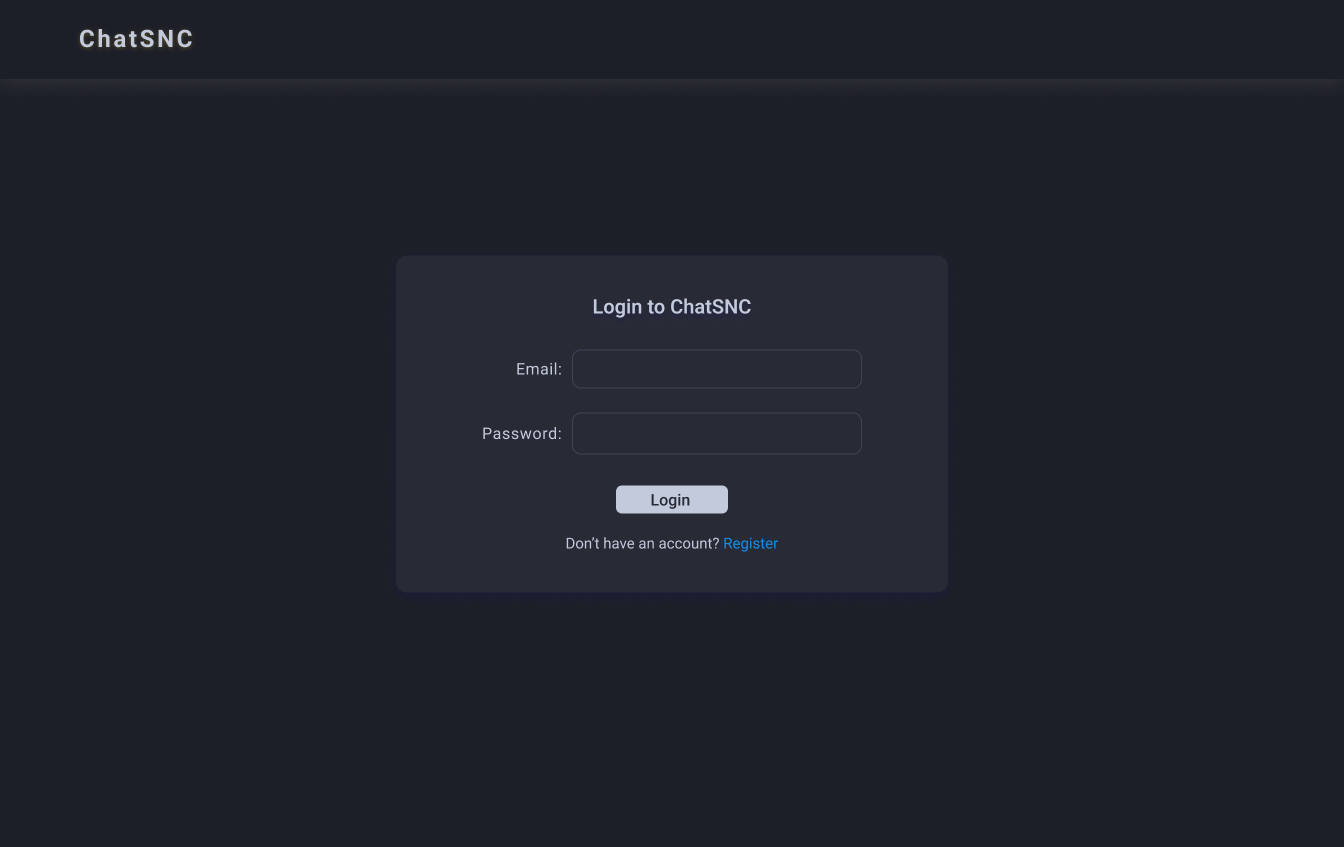
\includegraphics[width=.75\textwidth]{Login-UI.png}
  \caption{Login/Registration UI}\label{fig:login-ui}
\end{figure}

\begin{figure}[h]
  \centering
  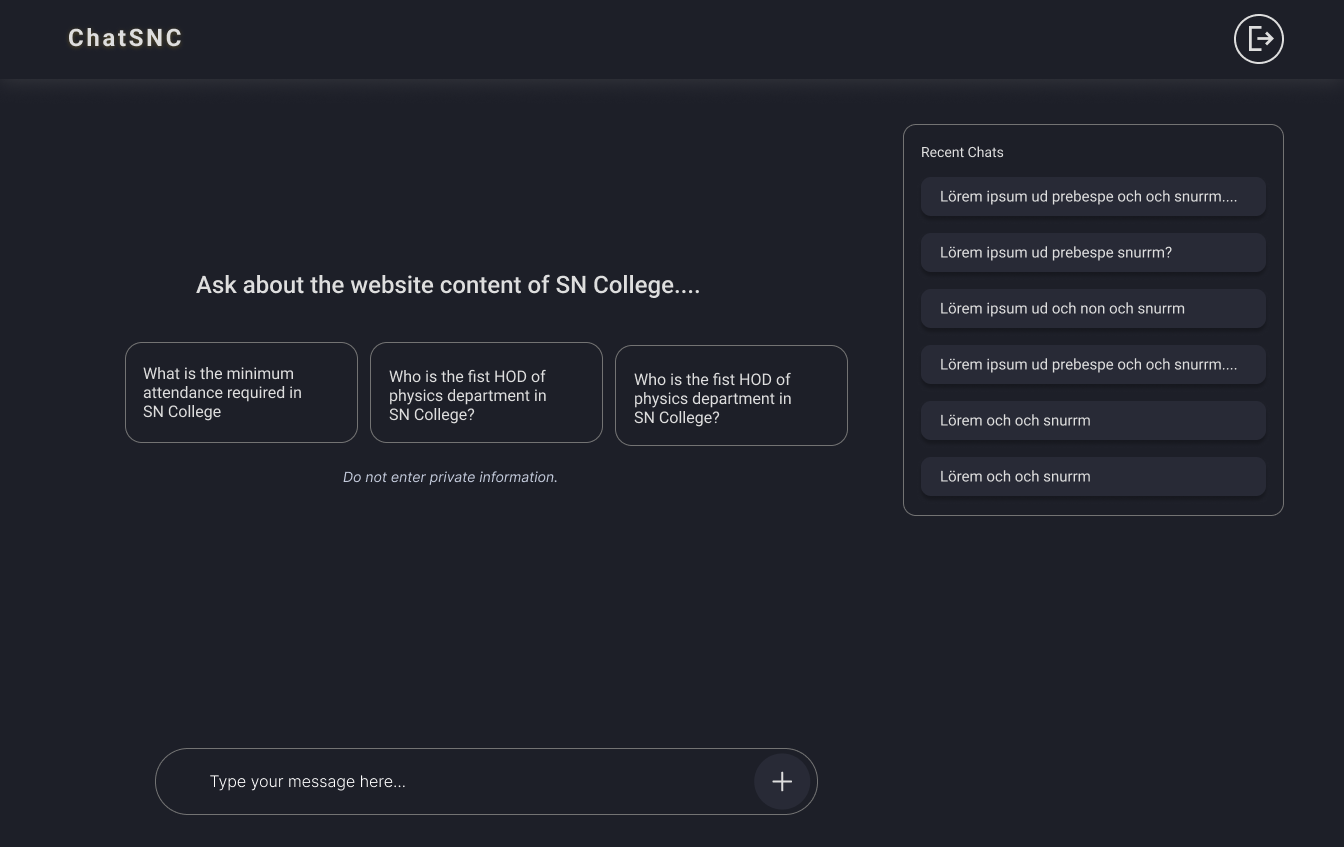
\includegraphics[width=.75\textwidth]{Chat-UI.png}
  \caption{Chat UI}\label{fig:chat-ui}
\end{figure}
\section{Algorithm Design}
\begin{figure}
  \centering
  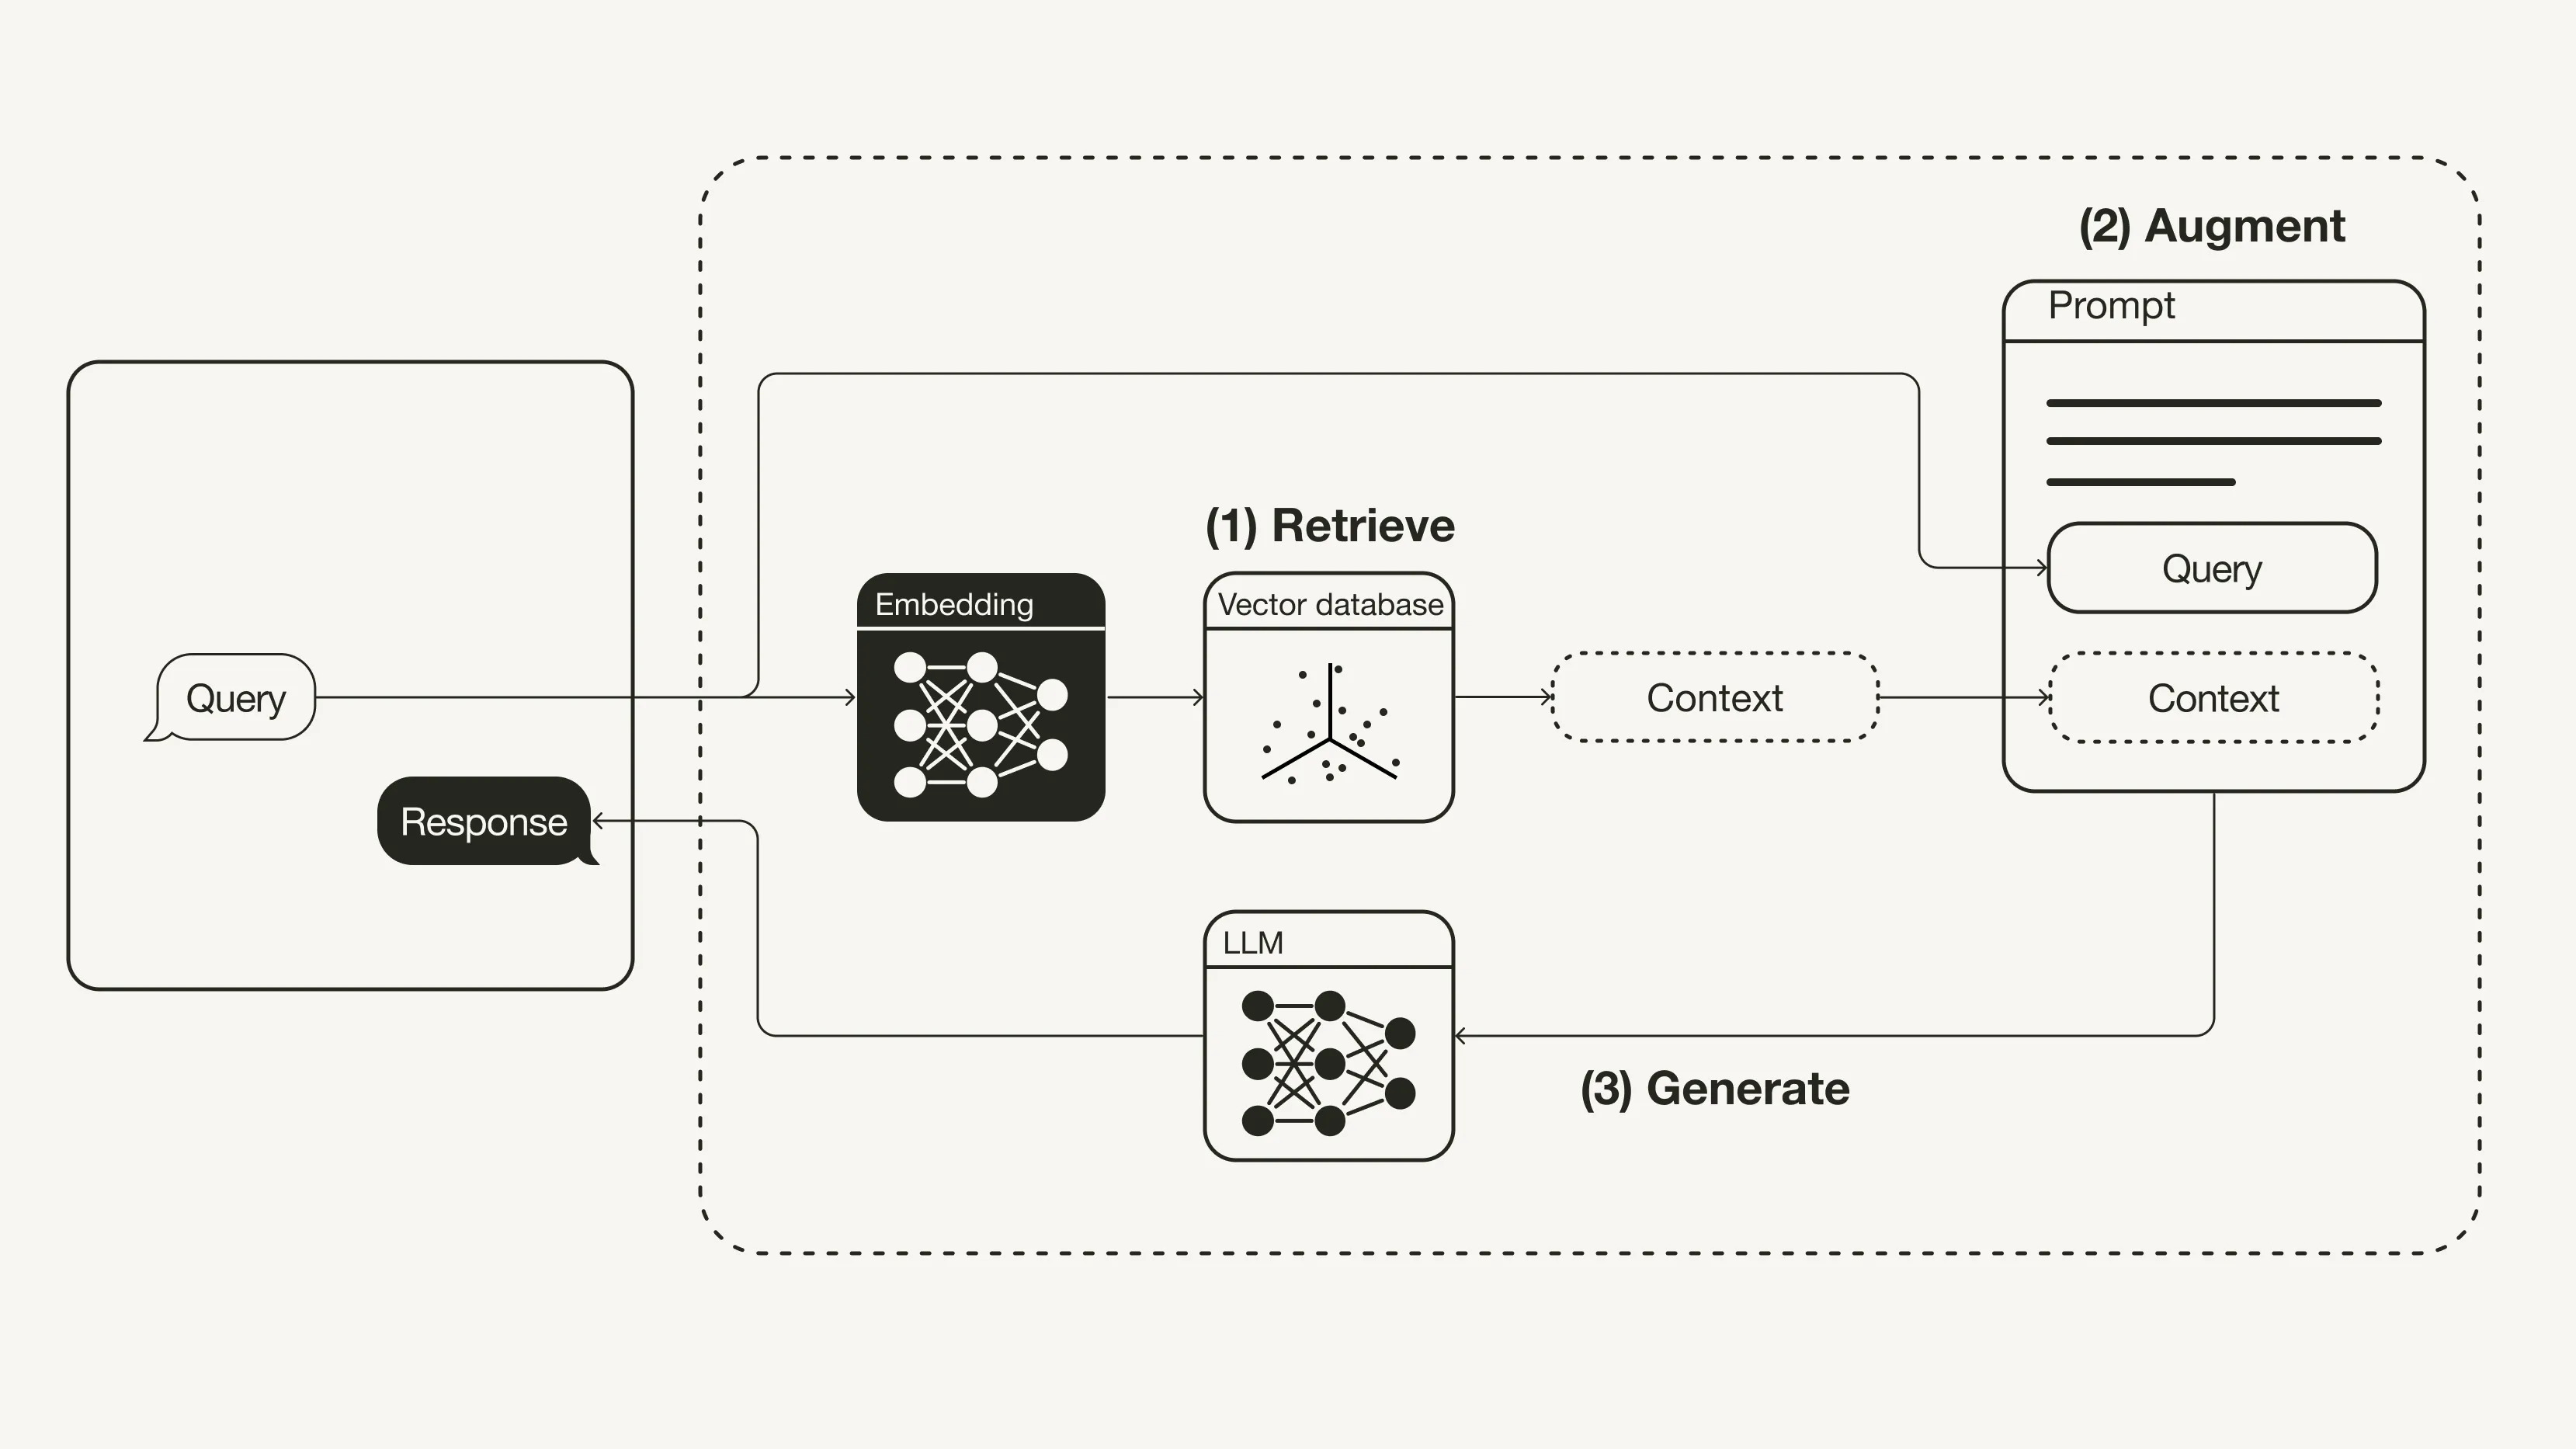
\includegraphics[width=.9\textwidth]{RAG-Algorithm.jpg}
  \caption{Retrieval Augmented Generation\cite{source-ref}}\label{fig:rag-algo}
\end{figure}
The core algorithm of this chatbot application is the Retrieval Augmented Generation (RAG) model, which combines the benefits of both retrieval-based and generative methods for chat generation. The RAG model is powered by GPT-3.5, a state-of-the-art language model known for its impressive text generation capabilities.
\\\\The RAG algorithm can be broken down into the following steps:
\begin{enumerate}
  \item \textbf{Query Encoding}: The user's input is first encoded into a query vector using a transformer-based encoder.
  \item \textbf{Document Retrieval}: The query vector is then used to retrieve relevant documents from a knowledge source. This is done using a technique called dense retrieval, where the query vector is compared with document vectors in the knowledge source to find the most relevant documents.
  \item \textbf{Context-Document Encoding}: The retrieved documents are concatenated with the original query to form a context-document pair. This pair is then encoded using another transformer-based encoder.
  \item \textbf{Response Generation}: Finally, a transformer-based decoder generates a response based on the context-document encoding. The decoder is autoregressive, meaning it generates the response one token at a time, using the previously generated tokens as context for the next token.
\end{enumerate}

The RAG model is particularly suited for open-domain question answering tasks, where the answer to a user’s query may be contained in any document in the knowledge source. By retrieving relevant documents before generating a response, the RAG model ensures that the generated responses are not only fluent and coherent, but also factually correct and informative.
\section{Database Design}
The database for this chatbot application is designed using PostgreSQL, a powerful, open-source object-relational database system. The database consists of two tables: \textit{users} and \textit{chats}.

\subsection{Users Table}


\begin{table}[h!]
  \centering
  \caption{users}
  \vspace*{10pt}
  \begin{tabular}{|c|c|c|c|}
    \hline
    Field Name & Data type & Constraints & Description\\ \hline
    id & int & Primary Key & Unique user identifier\\ \hline
    email & character varying & Not Null & User's email\\ \hline
    password & character varying & Not Null & User's password\\ \hline
    created\_at & timestamp & Not Null & Timestamp of user creation\\ \hline
  \end{tabular}
\end{table}

\subsection{Chats Table}

\begin{table}[h!]
  \centering
  \caption{chats}
  \vspace*{10pt}
  \begin{tabular}{|c|c|c|c|}
    \hline
    Field Name & Data type & Constraints & Description\\ \hline
    id & int & Primary Key & Unique chat identifier\\ \hline
    user\_id & int & Foreign Key & Identifier of the user \\ \hline
    history & character varying & Not Null & Chat history\\ \hline
    created\_at & timestamp & Not Null & Timestamp of chat creation\\ \hline
  \end{tabular}
\end{table}

